\chapter{Introduction}
This chapter details the scope of this dissertation and the context for which it exists in the area of computational fluids mechanics. An overview is given of turbulence modeling and the numerical methods developed for studying turbulence to provide insight into the quantities of interest within this dissertation and the choices of numerical methods used herein. Supercritical fluids are then defined and the challenges associated with studying them are presented. Important applications of supercritical carbon dioxide in particular are then provided to motivate the problem presented in this dissertation. Existing numerical studies on supercritical fluids are then reviewed to demonstrate how this dissertation fits into the current landscape of research and to emphasize the contribution the presented results make to the field. This chapter concludes with an outline of the dissertation, the goals of the dissertation, and the main contributions made through this work. 

\section{Turbulence}
Fluids are substances characterized by their continuous deformation under the effects of a shearing stress. Consequently, they are said to flow. Gases and liquids comprise the most common types of fluids, with familiar examples being found in the water we drink and the breeze felt on a warm summer day. Additionally, fluid flow can be categorized into different types based on certain defining flow characteristics. The main two classifications of note are laminar flow and turbulent flow.

Laminar flow is denoted by fluid particles having well-defined parallel trajectories of motion, or streamlines. Streamlines do not cross, meaning adjacent layers within the fluid flow by one another with little to no mixing. From a more generalized perspective, the flow appears to be smooth. In contrast to this, turbulent flow is characterized by its unpredictable and chaotic trajectories. Streamlines do cross resulting in swirls and eddies of varying length scales which induce mixing. Turbulent flow can be qualitatively described as being rough due to this high degree of fluctuation within the velocity and pressure fields present. This generalized description is depicted in Figure \ref{lam_vs_turb}.

\begin{figure}
\begin{center}
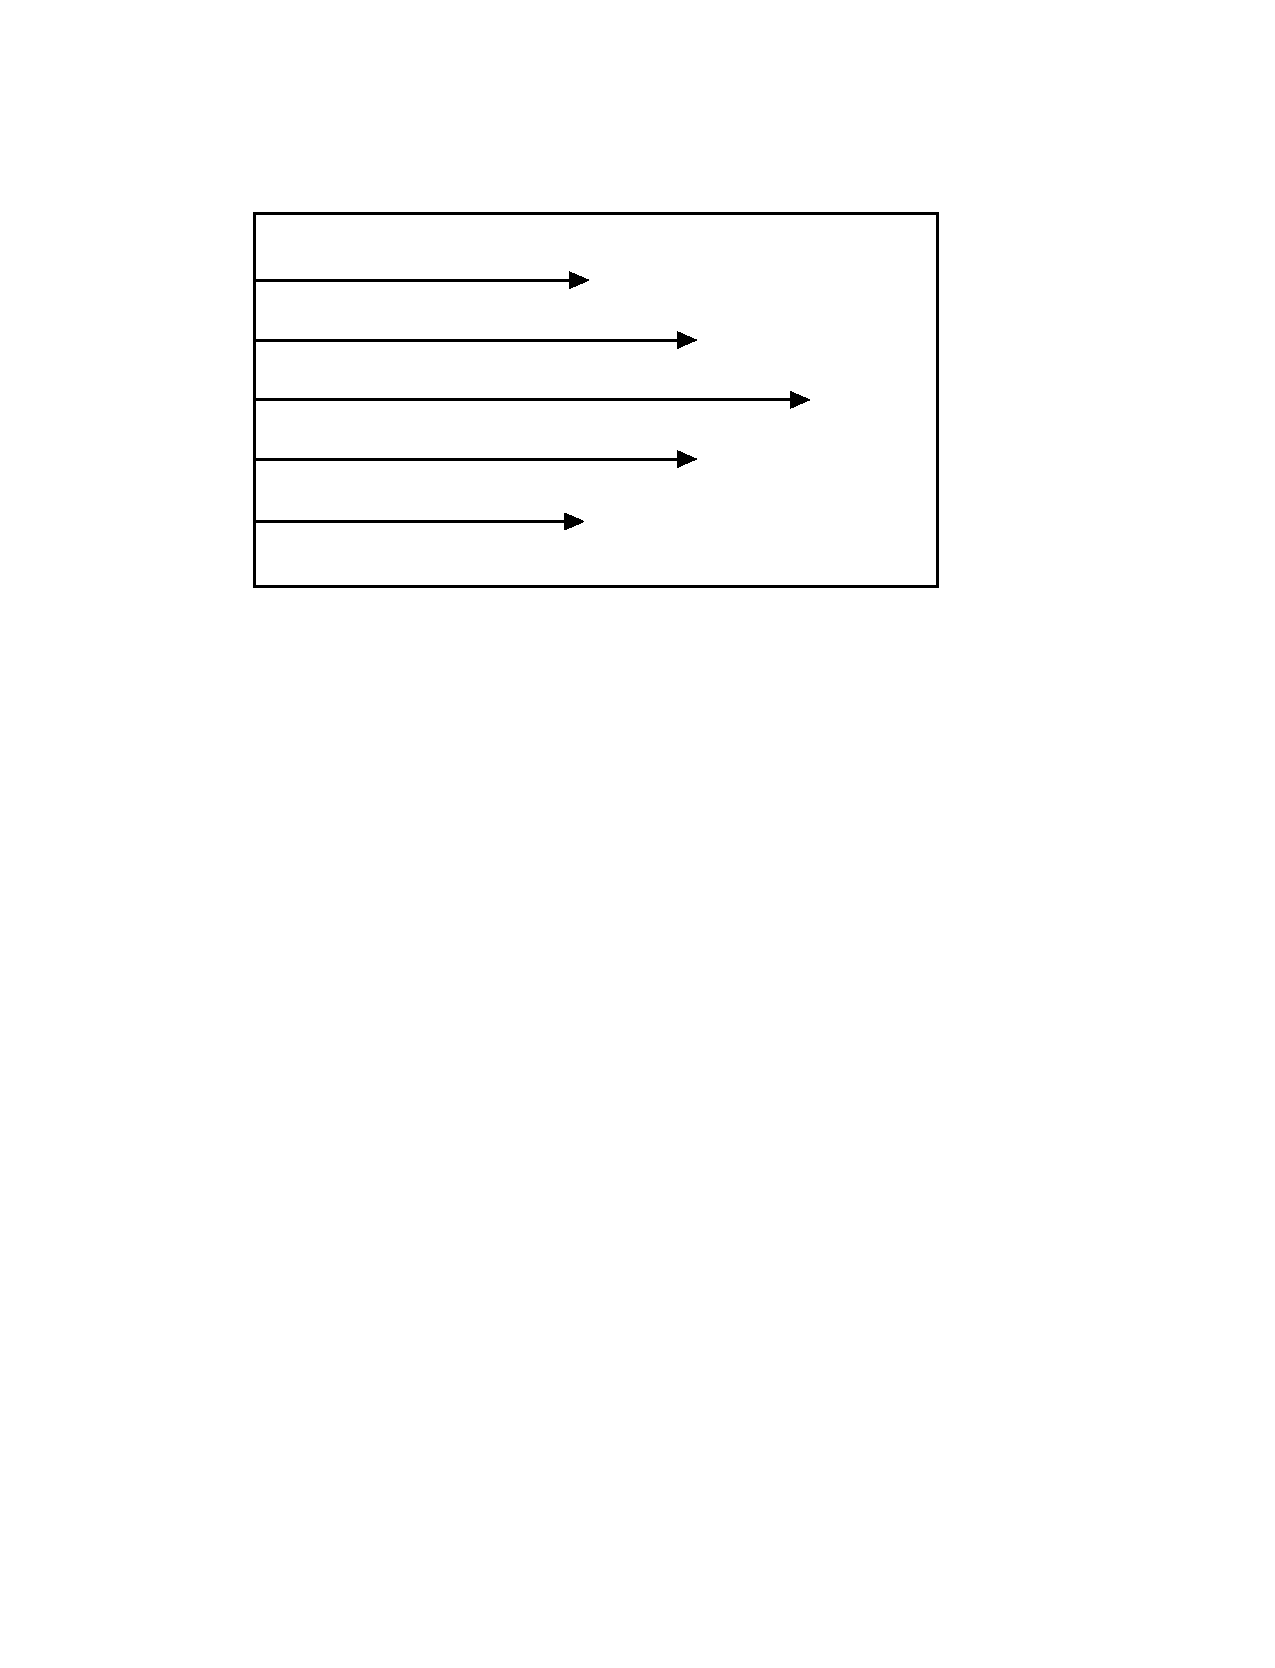
\includegraphics[scale=0.5]{figures/laminar}
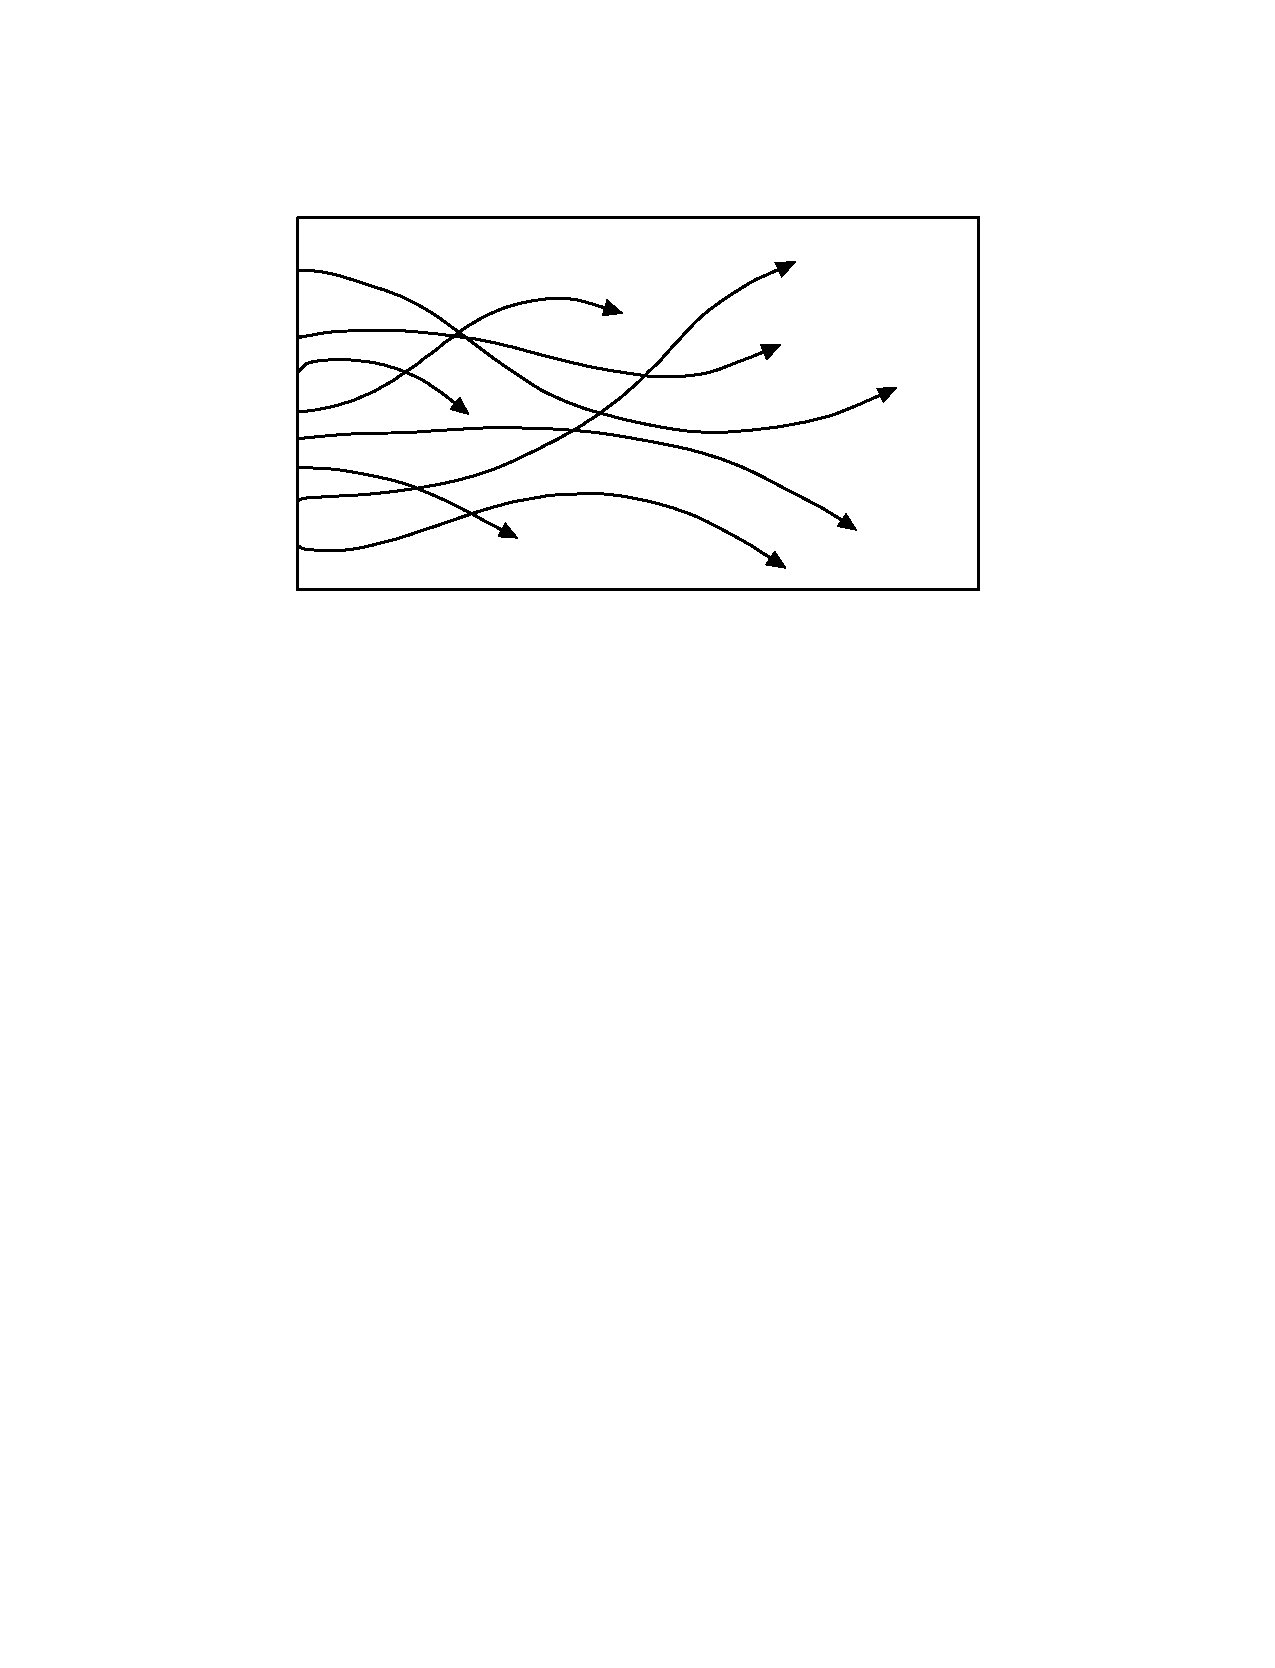
\includegraphics[scale=0.503]{figures/turbulent}
\end{center}
\caption{Example of streamlines in laminar (left) vs. turbulent (right) flow.}
\label{lam_vs_turb}
\end{figure}

The Reynolds number is a dimensionless value that can be used to distinguish laminar flow from turbulent flow. It is defined as follows:
\begin{equation}
\label{Reynolds_num}
\text{Re} = \frac{\rho u L}{\mu}
\end{equation}

\noindent where $\rho$ and $\mu$ are the density and dynamic viscosity of the fluid, respectively, $u$ is the flow velocity, and $L$ is a characteristic length scale associated with the given flow scenario (e.g. pipe diameter). As is demonstrated by the ratio in Equation \ref{Reynolds_num}, the Reynolds number measures the relative effects of inertial forces compared to viscous forces within a given flow scenario. A small Reynolds number signifies the dominance of viscous forces; fluid parcels moving in tandem want to ``stick together," resulting in the sheared flow and parallel trajectories seen in laminar flow. Turbulence is then characterized by a large Reynolds number, where inertial forces take precedence. Here, deviations within the laminar flow field result in lateral mixing between shear layers. This creates eddies and random trajectories that result in the chaotic motion of turbulent flow. 

This work focuses on the turbulent round jet and its associated dynamics in the context of supercritical fluids. The remainder of this section details a brief historical overview of turbulence modeling and numerical methods developed for studying turbulence in order to motivate the modeling and numerical choices made within this work.

\subsection{Historical Perspective}


\subsection{Numerical Approaches}


\section{Supercritical Fluids}

\subsection{Applications of Supercritical Carbon Dioxide}
Fluids also serve an important role in industry, proving useful in areas ranging from thermal management to energy production; steam turbines alone accounted for 45\% of electricity generation in the United States in 2021 \cite{US_elec_gen_stat}.  
\subsection{Overview of Current Numerical Landscape}






